\section{Implementation}
In this chapter, the aim is to:

\begin{itemize}
    \item Provide a detailed description of the Python code used to estimate cuffless blood pressure from PPG signals
    \item Discuss any changes or justifications made to the code

\subsection{Description of dataset}
As discussed in Chapter 3, the MIMIC Database includes data
recorded for 72 ICU patients, ranging from patient indexes '037' to '485'. Firstly, it was necessary to check which 
of these patients contained signal data for the PPG and ABP channels. As a result, the following patients were excluded from the dataset:
\begin{itemize}
    \item '037'
    \item '208'
    \item '209'
    \item '210'
    \item '222'
    \item '262'
    \item '291'
    \item '405'
    \item '413'
    \item '415'
    \item '450'
\end{itemize}\noindent Hence, there was now data available from 61 ICU patients.

\textcolor{red}{Why a subset? Why not all? If you're doing a split, explain this. Are you only using 8 patients out of the 90?}

\begin{table}[H]
    \centering
    \begin{tabular}{|cccc|}
    \hline
    \textbf{Patient Number} & \textbf{Gender} & \textbf{Age} & \textbf{Health issue faced by the patient} \\ \hline
    224 & Male   & 21 & Sepsis                                  \\
    225 & Male   & 73 & Pulmonary edema                         \\
    230 & Female & 75 & Cardiac Heart Failure/Pulmonary edema   \\
    232 & Male   & 68 & Myocardial infarction/Cardiogenic shock \\
    235 & Female & 67 & Myocardial infarction/Cardiogenic shock \\
    240 & Male   & 68 & Angina                                  \\
    252 & Male   & 52 & Respiratory Failure                     \\
    255 & Male   & 67 & Cardiac Heart Failure/Pulmonary edema   \\ \hline
    \end{tabular}
    \caption{Characteristics of the patients from the MIMIC-I database}
    \label{tabPatients}
    \end{table}


\subsection{Extracting the ground truth blood pressure values}
The ground truth Systolic and Diastolic blood pressure values are calculated by taking the respective 
maxima and minima of the arterial blood pressure signal within each window of the signal.




\subsection{Signal preprocessing steps}


\subsection{Windowing of PPG and ABP data}

\subsection{Convolutional Neural Network (CNN) model}

\textcolor{red}{What type of information should the reader gather from this figure? It needs explaining and annotations/labelling.}

\begin{figure}[H]
    \centering
    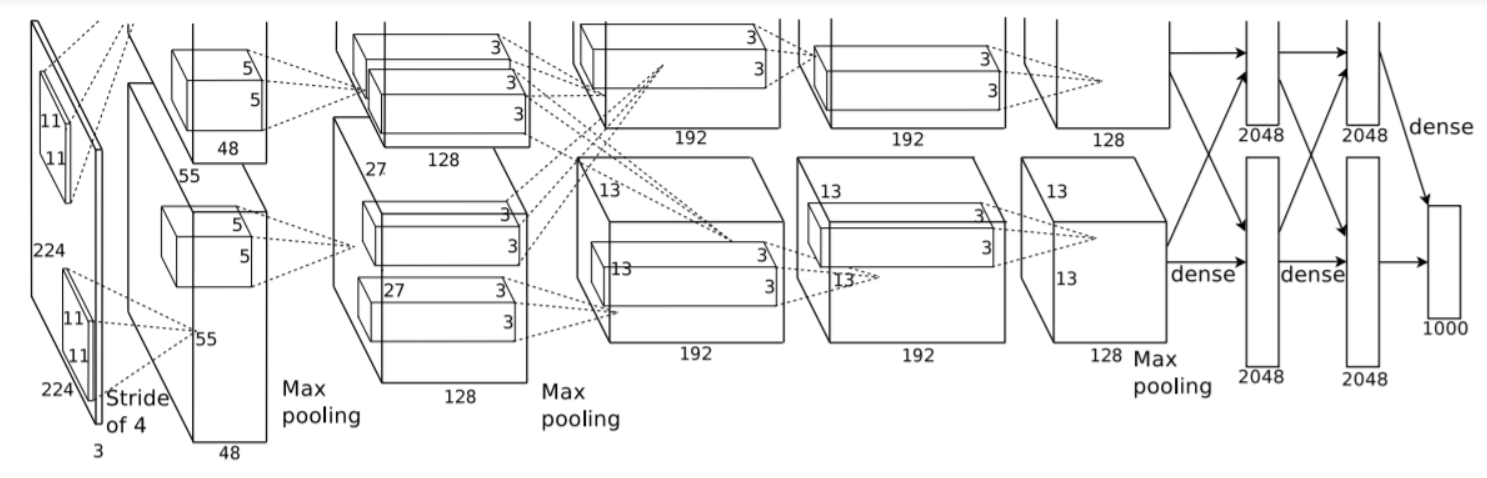
\includegraphics[width=10cm,height=10cm,keepaspectratio]{Implementation/alexnetArch.png}
    \caption{Overview of the AlexNet architecture}
    \label{alexnetArch}
\end{figure}



\subsection{ResNet model}


%\subsection{Potentially for appendix: Description of other models the transformer is compared with}
